\documentclass[11pt,a4paper]{article}
\usepackage[margin=24mm]{geometry}
\usepackage{graphicx,booktabs,tabularx}
\usepackage[hidelinks]{hyperref}
\title{ReVive\\\large Explainable Financial Anomaly Detection\\UCS503P Final Project Report}
\author{Aakriti Sharma (1024030430) \and Koena (1024030831) \and Mayur Goyal (1024030828)}
\date{Thapar Institute of Engineering and Technology\\25 November 2026}
\begin{document}
\renewcommand{\labelitemi}{\(\bullet\)}
\maketitle
\begin{abstract}
ReVive prioritizes suspicious windows of financial transactions and exposes repair-error explanations in a deployed Streamlit dashboard. In a chronological experiment on 8,000 transactions, its average precision was 0.9681. Validation-calibrated thresholds reduced the number of alerts from 626 to 338 on the same 631 test windows while preserving recall in this experiment.
\end{abstract}

\section{Problem and scope}
A reviewer needs a ranked workload and evidence for investigating an alert. ReVive implements batch ingestion, anomaly scoring, triage, explanations, and alert persistence. The deployed dashboard accepts a public transaction CSV or generates synthetic demo data. A labeled test window is positive if it contains at least one labeled fraud transaction. The interface reports window-level results and is an academic decision-support prototype.

\section{Requirements and design}
\begin{itemize}
\item Accept numeric transaction features and an optional binary label. Reject invalid feature values with a visible message.
\item Train on normal windows, benchmark on chronological held-out windows, and record run settings.
\item Prioritize alerts using validation-calibrated or user-controlled cutoffs. Explain flagged windows with feature repair error and the peak error timestep.
\item Persist alert metadata in SQLite and show historical alerts in the dashboard.
\end{itemize}
\begin{center}
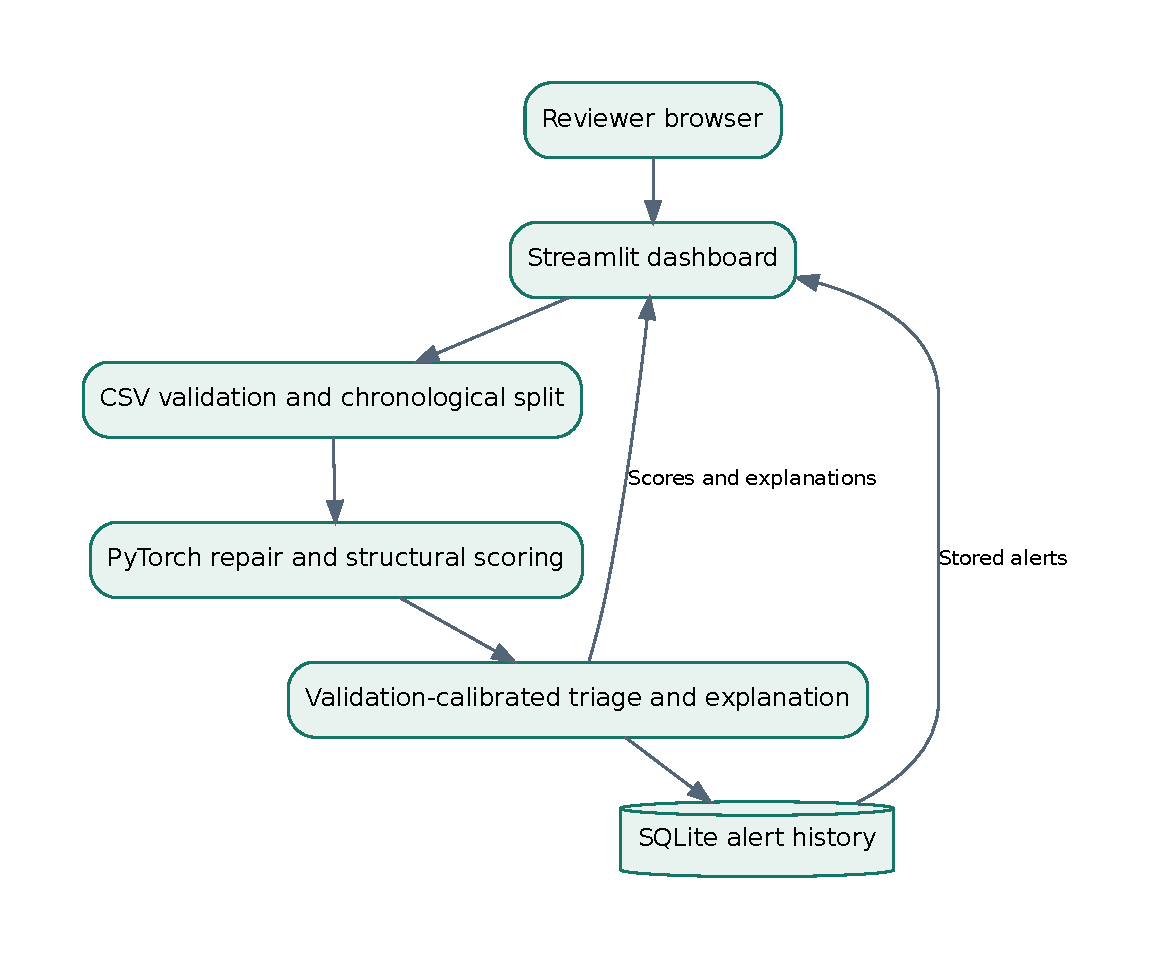
\includegraphics[height=0.32\textheight,width=0.93\linewidth,keepaspectratio]{architecture.pdf}
\end{center}

\section{Implementation and evolution}
The dashboard calls the data preparation, PyTorch model, scoring, baseline, explanation, and triage modules in-process. Uploaded rows are ordered by time when available. Time is excluded from model features. The final build splits rows before windowing and fits preprocessing only on normal training rows. This corrects the prototype's full-input scaling and prevents adjacent windows from crossing partition boundaries. The normal training and validation windows retain original row adjacency.

The model independently implements the repair approach in JuRe \cite{jure}: a compact depthwise-separable residual block learns to repair Gaussian noise and channel masking. Inference uses amplitude, first-difference, trend, and correlation discrepancies. Scores are standardized using the normal training reference. The 95th and 99th percentiles of normal validation scores define the default Review Needed and High Risk cutoffs. That validation partition also supports early stopping.

Each alert shows triage, an anomaly score, and the features with the largest absolute repair error. This attribution describes repair discrepancy. The SQLite table records window index, score, tier, top feature, contribution, and timestamp.

\section{Held-out evaluation}
We used the first 8,000 rows of the ULB credit-card dataset \cite{ulb}. The chronological row split was 4,320 training, 480 validation, and 3,200 test rows. Window length was 50 and stride was 5. Hidden width was 64, seed was 42, and training stopped at six of ten allowed epochs. There were 835 normal training windows, 87 normal validation windows, and 631 test windows. Of the test windows, 135 were positive. Isolation Forest and LOF were fitted on flattened training windows and evaluated on the same test windows. LOF caps its reference pool at 3,000 windows.

\begin{center}
\begin{tabular}{lrr}
\toprule
Detector & Average precision & ROC-AUC\\
\midrule
ReVive & 0.9681 & 0.9894\\
Isolation Forest & 0.3249 & 0.6646\\
Local Outlier Factor & 0.4914 & 0.8161\\
\bottomrule
\end{tabular}

\vspace{1em}
\begin{tabular}{lrrrr}
\toprule
Policy & Flagged & Alert rate & Precision & Recall\\
\midrule
Default (2.0 / 4.0) & 626 & 99.21\% & 21.57\% & 100\%\\
Calibrated (4.7970 / 5.0895) & 338 & 53.57\% & 39.94\% & 100\%\\
\bottomrule
\end{tabular}
\end{center}

Both policies used the same test scores. Calibration removed 288 alerts and retained all 135 positive windows in this run. Average precision describes ranking quality while precision and recall in the second table describe the selected review cutoff.

\section{Verification}
\begin{center}
\begin{tabularx}{\linewidth}{@{}lXX@{}}
\toprule
Check & Expected behavior & Observed behavior\\
\midrule
Labeled CSV & Complete benchmark & All three detector rows appeared\\
Invalid feature & Reject a nonnumeric field & Numeric feature error displayed\\
Triage & Compare cutoffs on the same scores & Alert counts were 626 and 338\\
Explanation & Show feature errors and peak position & Flagged-window explanation rendered\\
Persistence & Reload alerts in a fresh app session & All 338 calibrated alerts reappeared\\
Seeded repeat & Match the displayed tables & Both tables matched at displayed precision\\
\bottomrule
\end{tabularx}
\end{center}
See the repository's \texttt{code/VERIFICATION.md} for dependency versions and input checksum.

\section{Deployment and limitations}
The application is available at \url{https://revive2627.streamlit.app/}. The repository and project documentation are linked from the course fork. Use synthetic demo data or a public CSV during evaluation. The hosted SQLite file is shared inside the running instance and may reset after redeployment. This delivery has a single Streamlit process that runs training and scoring.

The experiment covers one chronological subset, and overlapping windows share observations. Adjacent transactions may belong to different cardholders. The anonymized PCA features constrain business interpretation, and a 53.57\% flag rate remains considerable. Future evaluation can use more chronological holdouts, separate calibration data, and threshold selection based on an explicit review budget.

\begin{thebibliography}{9}
\bibitem{jure} K.-K. Ozer, R. Ebeling, and M. Enzweiler. \emph{Back to Repair: A Minimal Denoising Network for Time Series Anomaly Detection}. arXiv:2604.17388, 2026. \url{https://arxiv.org/abs/2604.17388}
\bibitem{ulb} Universite Libre de Bruxelles Machine Learning Group. \emph{Credit Card Fraud Detection dataset}. \url{https://www.kaggle.com/datasets/mlg-ulb/creditcardfraud}
\end{thebibliography}
\end{document}
